\vspace{-1.5cm}
\small
\textbf{The results in this chapter are published as:}
\vspace{0.05 cm}

% We cite the paper with fontsize 10
\fullcite{abella2024dynamics}
\normalsize
\vspace{0.5 cm}

\section{Introduction}

\section{Data}

We use the dataset, mentioned in section \ref{sec:Datasets}, of listings published on the portal \texttt{Idealista.com} \cite{idealista}. The dataset covers a 2-year time period, from January 2017 to December 2018 and it comprises a comprehensive collection of online listings georeferenced with their (lat, long) coordinates in the Spanish provinces of Balearic Islands, Barcelona, and Madrid. These listings were posted by real estate agencies for renting or selling residential properties. Posted listings by private individuals are not included into the dataset.

Each listing contains a set of attributes such as the price, the surface area, the real estate agency that posted it, its location and the dates of both the publication and the removal of the listing. The dataset also contains information about the type of property (e.g. flat, house, etc.), what allowed us to filter rural parcels and commercial properties.

\section{Listings dynamics}

\begin{figure}
    \label{fig:active_adds}
    \centering
    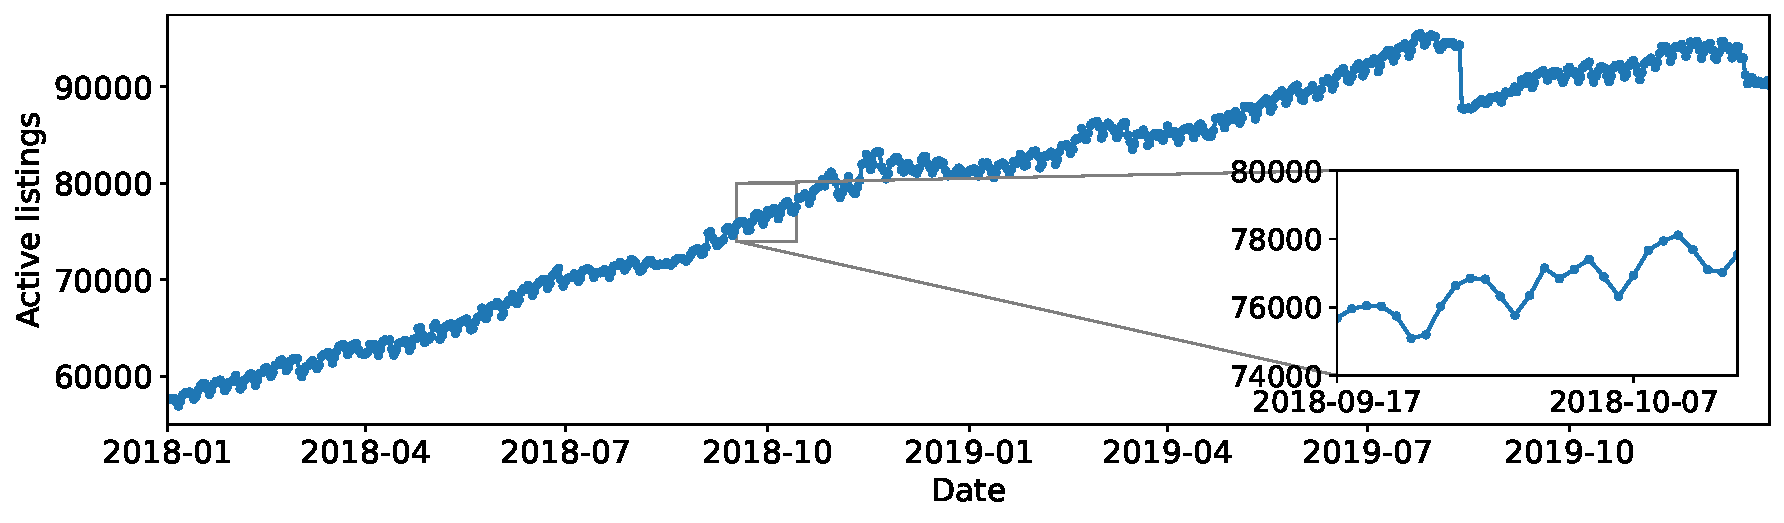
\includegraphics[width =\textwidth]{Figs/Idealista_dynamics/active_adds.pdf}
	\caption[Active listings evolution.]{Daily number of active listings during the period 2018 - 2020 for the Barcelona province. The inset shows a zoomed view to a 1 month period, where the weekly patterns are more evident.}
\end{figure}

\begin{figure}
    \label{fig:panel_time}
    \centering
    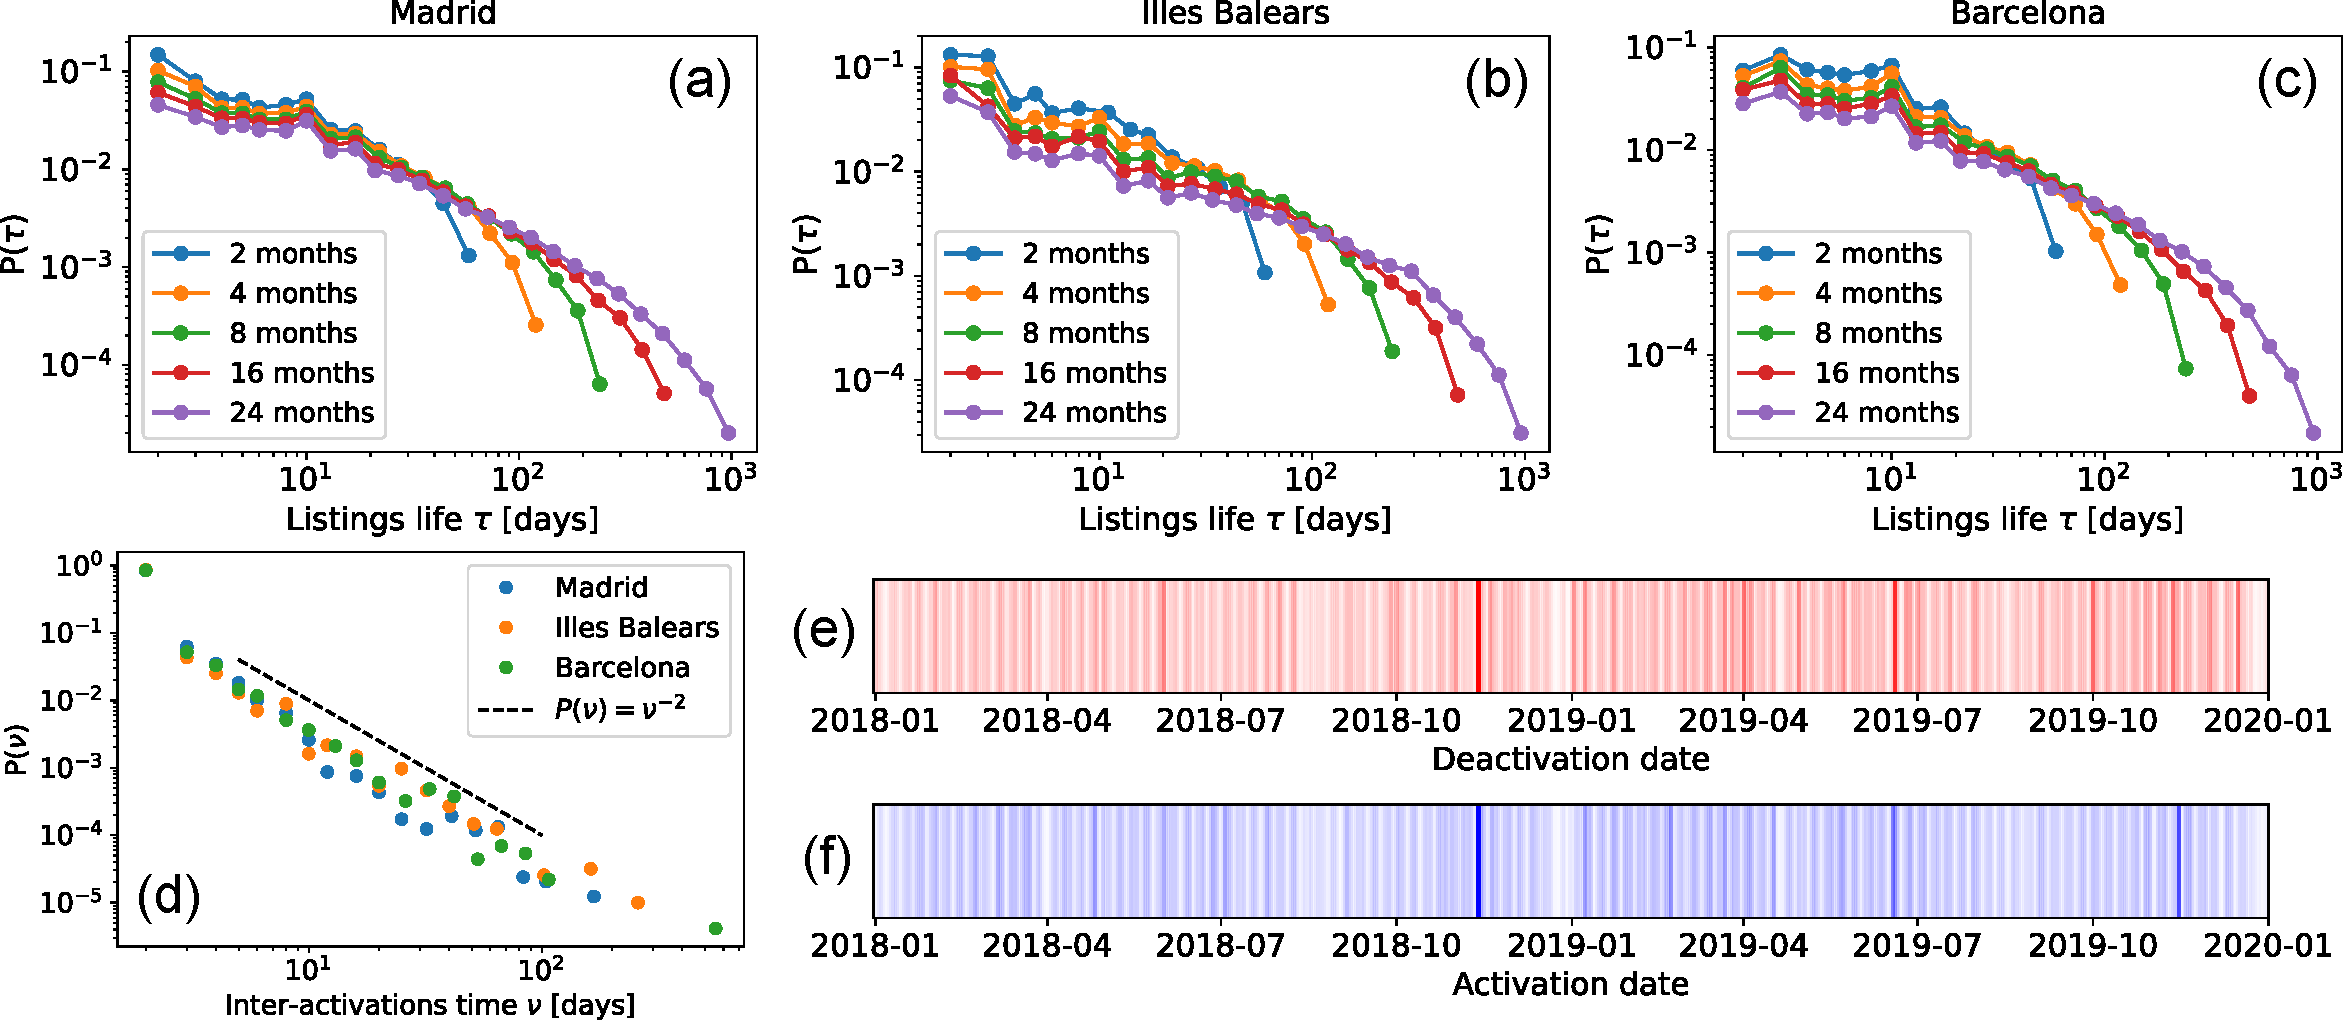
\includegraphics[width =\textwidth]{Figs/Idealista_dynamics/panel_time.pdf}
	\caption[Temporal statistics of the listing dynamics.]{Temporal statistics of the listing dynamics. Listings life (time posted in the platform) distribution for different time windows at Madrid \textbf{(a)}, Barcelona \textbf{(b)} and Balearic Islands \textbf{(c)}. Different colors indicate different time windows. \textbf{(d)} Inter-activations time distribution for the 3 regions. Different colors indicate different region or province. The dashed black line shows a $\nu^{-2}$ power-law distribution. \textbf{(e)} and \textbf{(f)} show the bar sequence of the adds deactivations and activations, respectively, for the Balearic Islands market. The color intensity indicates the number of adds.}
\end{figure}

\section{Agencies dynamics}

\subsection{Preferential attachment}

\begin{figure}
    \label{fig:panel_degree}
    \centering
    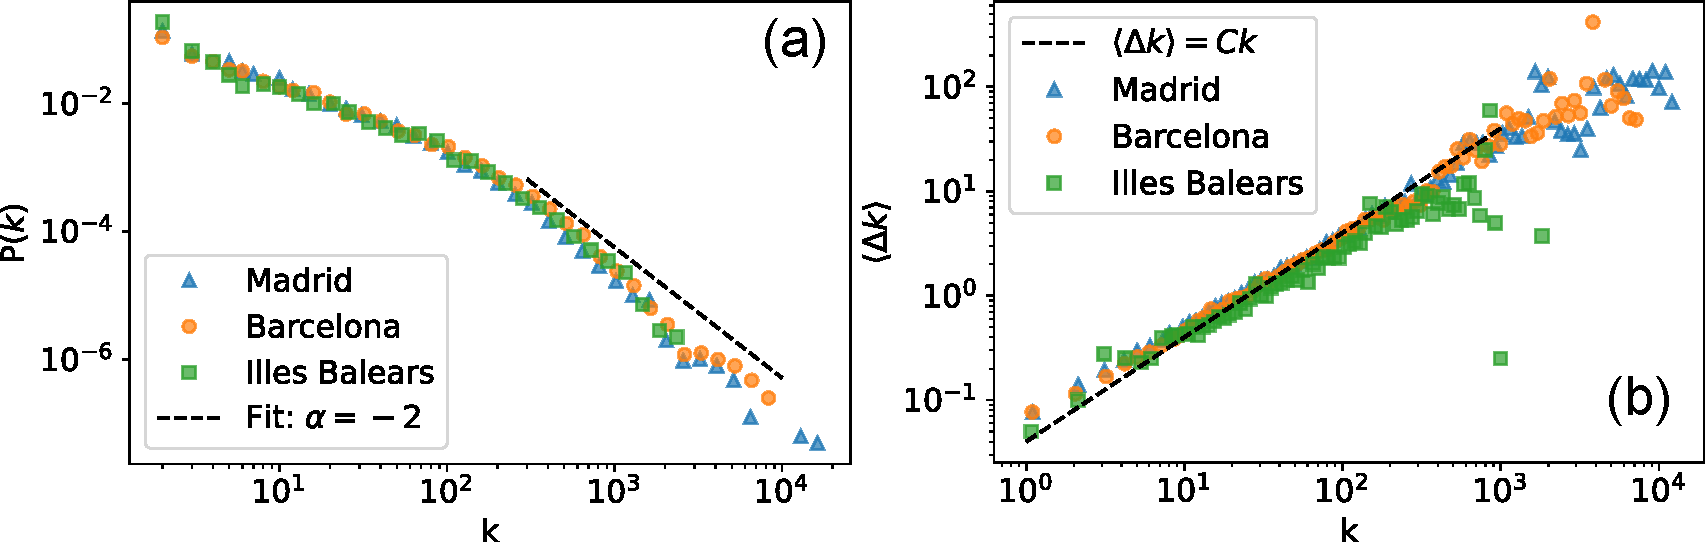
\includegraphics[width =\textwidth]{Figs/Idealista_dynamics/panel_degree.pdf}
	\caption[Preferential attachment to agencies.]{Preferential attachment to agencies. \textbf{(a)} Degree distribution of the agencies in the 3 regions. \textbf{(b)} Average degree increase of an agency as a function of the degree (listings posted) of the agency previously to the attachment. For both plots, different colors and markers indicate different regions or provinces. In \textbf{(a)}, the black dashed line shows a power-law distribution with exponent $\alpha  =-2$, and in \textbf{(b)} shows a linear increase with fitted slope $C = 0.04$.}
\end{figure}

\subsection{Price correlations}

\begin{figure}
    \label{fig:sigma_price}
    \centering
    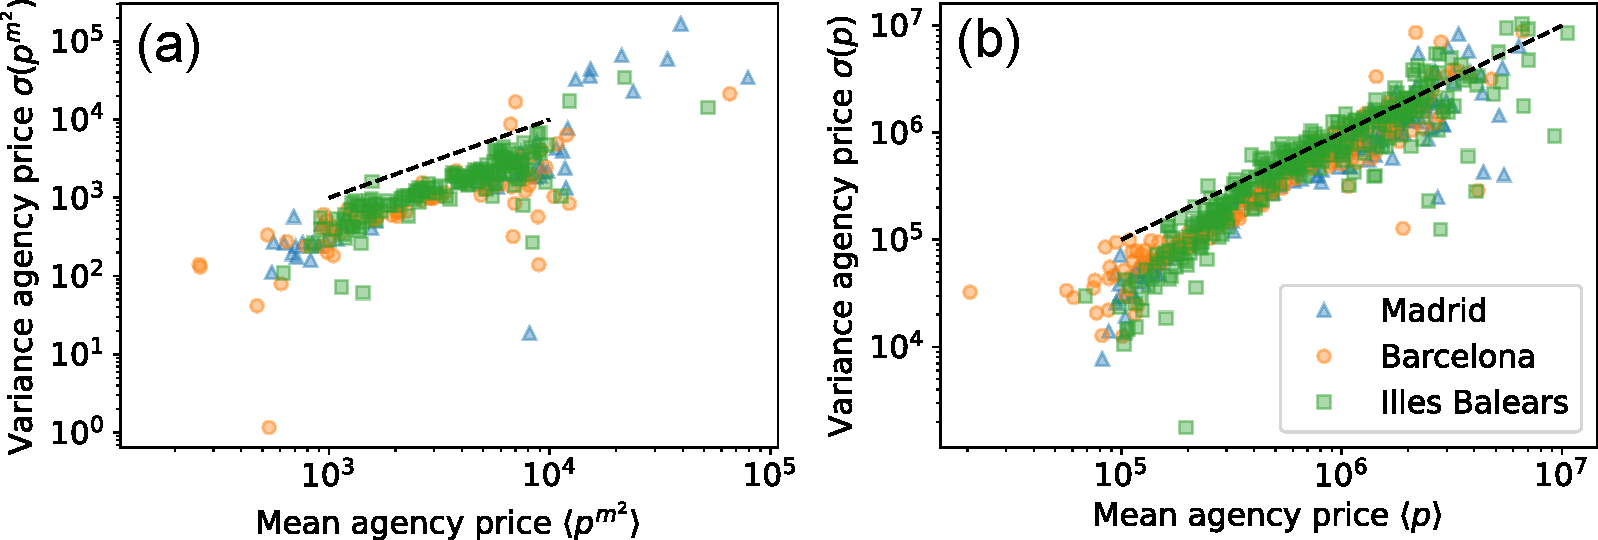
\includegraphics[width =\textwidth]{Figs/Idealista_dynamics/labeled_sigma_price.pdf}
	\caption[Variance of the agency price vs mean agency price.]{Variance of the listings posted by an agency as a function of its mean price for the price per square meter \textbf{(a)} and the total price \textbf{(b)}. Different colors and markers indicate different regions or provinces. The black dashed line shows a linear fit with $\sigma = p^{{m}^2}$ for both plots.}
\end{figure}

\begin{figure}
    \label{fig:panel_price}
    \centering
    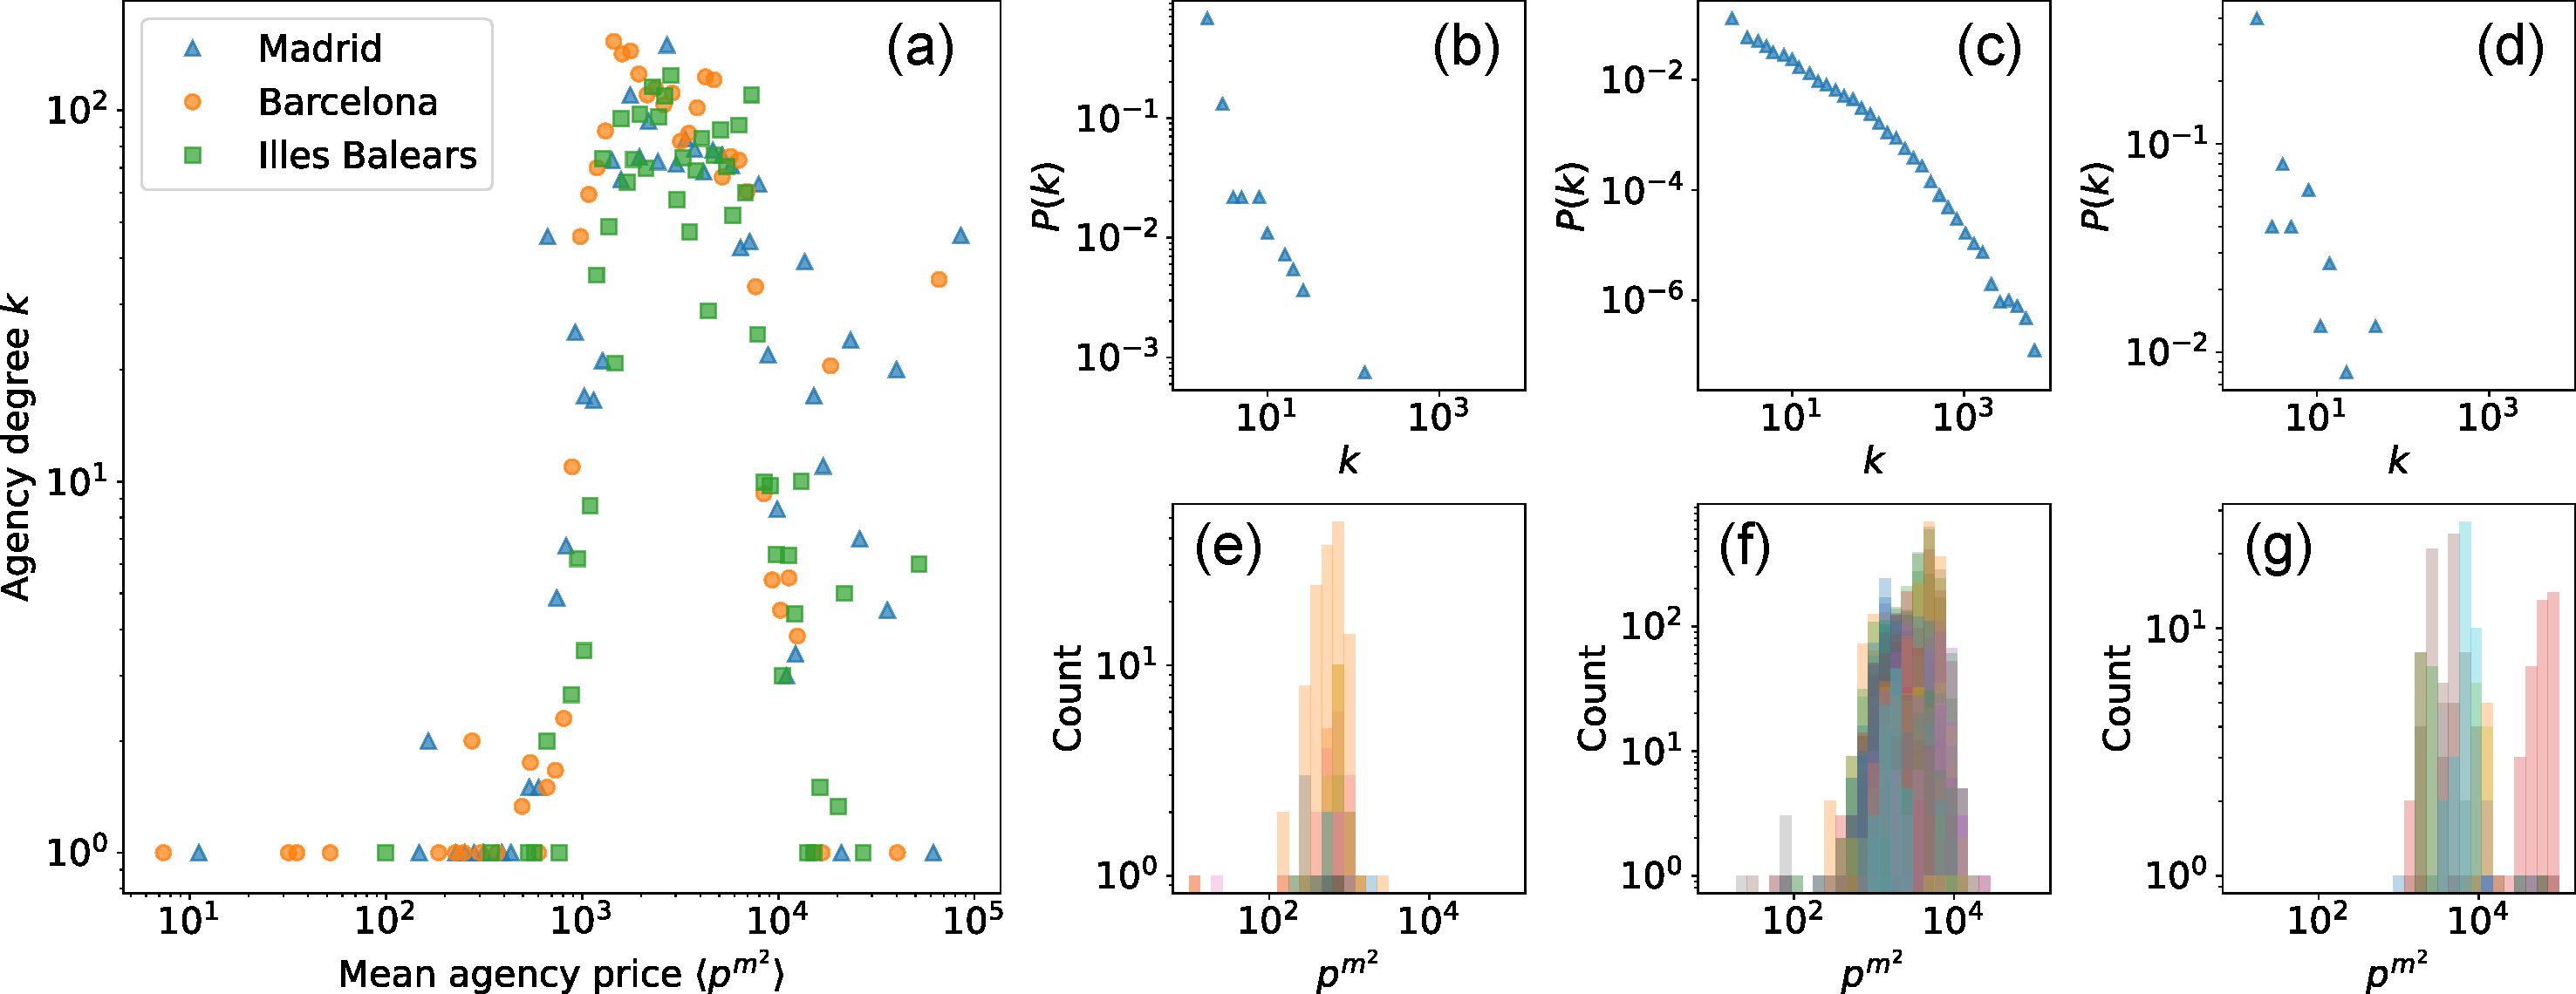
\includegraphics[width =\textwidth]{Figs/Idealista_dynamics/panel_price.pdf}
	\caption[Price segmentation by the degree.]{\textbf{(a)} Average degree (number of listings) of an agency as a function of its mean price per square meter. Different colors and markers indicate different regions or provinces. Degree distribution of the agencies at the different price ranges: \textbf{(b)} $p^{{m}^2} < 800 \euro / m^2$, \textbf{(c)} $800 \textup{\euro}  / m^2 < p^{{m}^2} < 10^4 \textup{\euro}  / m^2$, and \textbf{(d)} $p^{{m}^2} > 10^4 \textup{\euro}  / m^2$.}
\end{figure}

\begin{figure}
    \label{fig:attach_price}
    \centering
    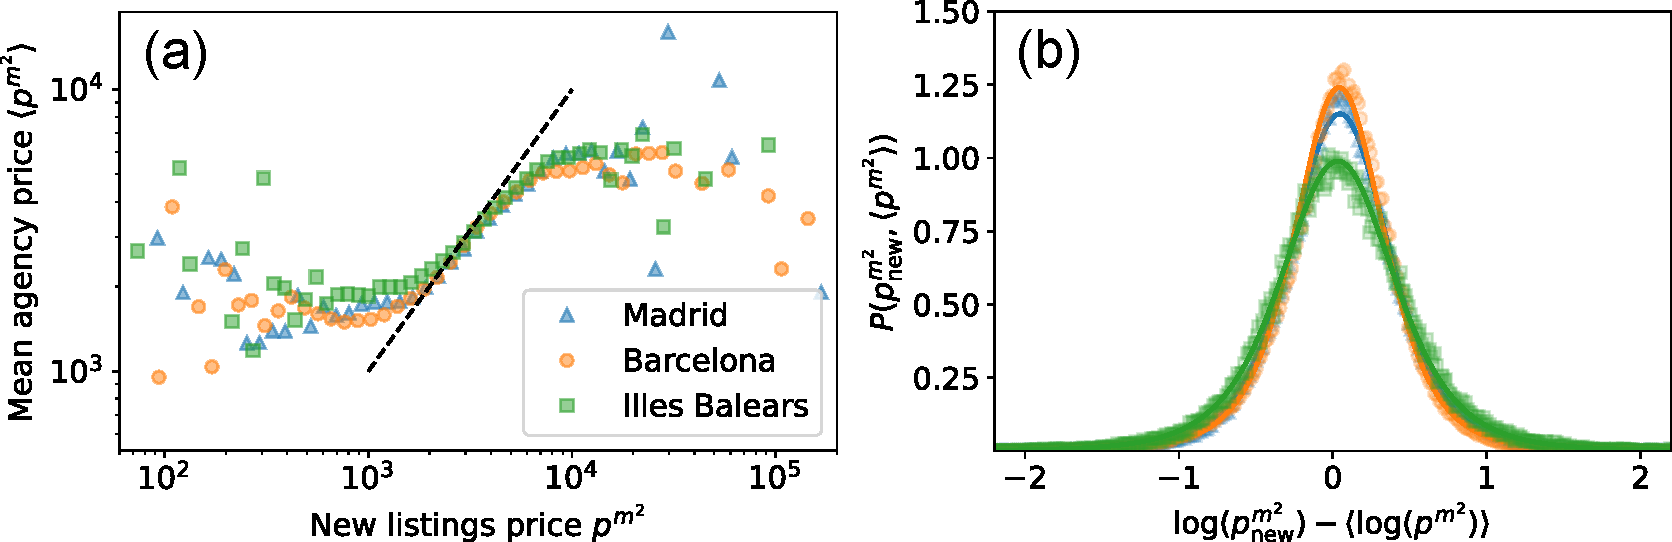
\includegraphics[width =\textwidth]{Figs/Idealista_dynamics/panel_attach_price.pdf}
	\caption[.]{ . }
\end{figure}

\subsection{Specialization}

\begin{figure}
    \label{fig:distance_panel}
    \centering
    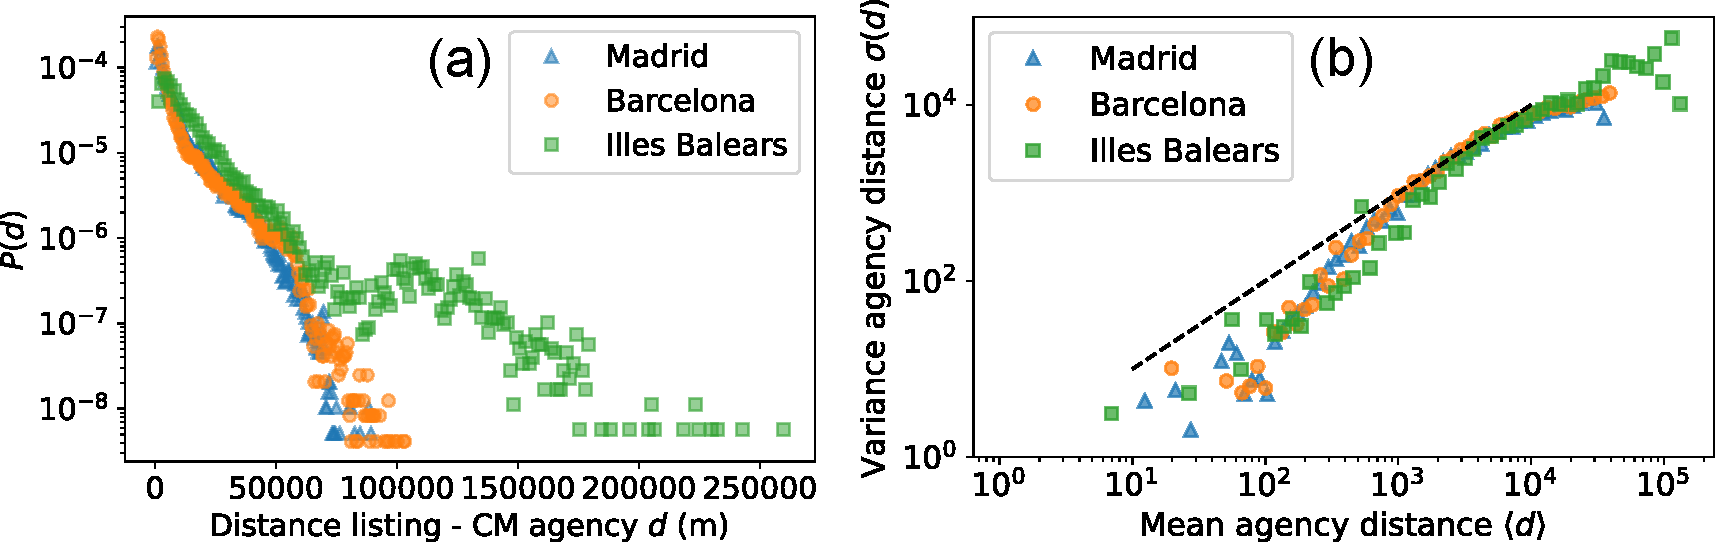
\includegraphics[width =\textwidth]{Figs/Idealista_dynamics/distance_panel.pdf}
	\caption[.]{ . }
\end{figure}

\begin{figure}
    \label{fig:distance_attach}
    \centering
    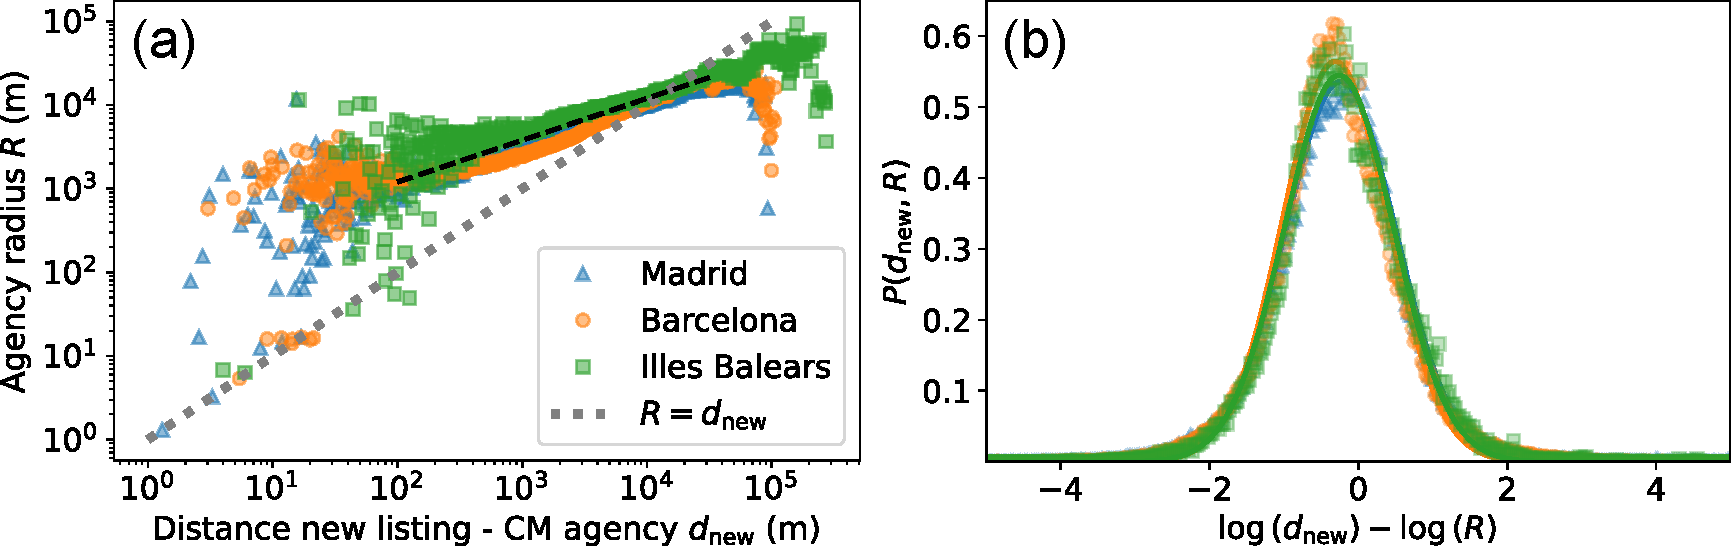
\includegraphics[width =\textwidth]{Figs/Idealista_dynamics/distance_attach.pdf}
	\caption[.]{ . }
\end{figure}

\section{Conclusions}












